\documentclass[a4paper, twoside]{article}
\usepackage[margin=12mm, bottom=0.75in, verbose]{geometry}
\usepackage{graphicx}
\usepackage{here, multicol, fancyhdr}
\usepackage{charter, courier}
\usepackage[OT1,T1]{fontenc} %use TeX encoding then Type 1.
\usepackage[protrusion=true, expansion=true]{microtype} % Better typography
\usepackage[english]{babel} % English language/hyphenation
\usepackage[utf8]{inputenc}
\usepackage{amsmath,amsfonts,amsthm} % Math packages
\usepackage{lettrine} % dropped capital letter
\usepackage{booktabs} % Horizontal rules in tables
\usepackage[small, labelfont=bf, up, textfont=up]{caption}
\usepackage[rgb]{xcolor} % Should be CMYK if supported by the system

% Colours by PRACE graphics guidelines
%\definecolor{prace-darkblue}{rgb}{0.1, 0.19, 0.48} % 25, 49, 123
%\definecolor{prace-lightblue}{rgb}{0.52, 0.81, 0.94} %132, 206, 239
% Colours by SoHPC logo pipette measurements
\definecolor{prace-orange}{rgb}{1.0,0.42, 0.1} % 255, 107, 25
\definecolor{prace-darkblue}{rgb}{0.08, 0.31, 0.58} % #155195 = 21,81,149
\definecolor{prace-lightblue}{rgb}{0.32, 0.73, 0.93} % #51bbed = 81,187,237
\newcommand{\highlight}[1]{\textcolor{prace-orange}{#1}}
\definecolor{link}{rgb}{0.1, 0.19, 0.48}

\usepackage{sectsty} % Enables custom section titles
\allsectionsfont{\large\color{prace-orange}\usefont{OT1}{phv}{m}{n}}
\usepackage[superscript,biblabel]{cite}
\usepackage{calc,float,wrapfig}\restylefloat{figure}

\usepackage[colorlinks=true, linkcolor=link, anchorcolor=link,citecolor=link,
filecolor=link, menucolor=link,urlcolor=prace-darkblue]{hyperref}

%\pagestyle{empty}
% Do not enable page numbering below as it will be inserted by the publication
%\pagestyle{fancy}\fancyhf{}\renewcommand{\headrulewidth}{0pt}\renewcommand{\footrulewidth}{0pt}\fancyfoot[C]{\colorbox{orange}{\raisebox{0mm}[4mm][7mm]{\textcolor{white}{\usefont{OT1}{phv}{m}{n}\selectfont~\thepage~}}}}
%To automatically convert Inkscape SVG into PDF or EPS use:
% pdflatex -synctex=1  --enable-write1 sohpc-template.tex
\newcommand{\includegraphicsvg}[2][]{%
  \ifnum\pdfstrcmp{\pdffilemoddate{./#2.svg}}%
  {\pdffilemoddate{../gen/#2.pdf}}>0%
  {\immediate\write18{inkscape -z -D --file=./#2.svg %
      --export-pdf=#2.pdf --export-eps=#2.eps %
      --export-area-drawing}}\fi%
  \includegraphics[#1]{#2}%
}

\graphicspath{{img/}}

% http://tex.stackexchange.com/questions/59166/span-column-in-a-multicols-environment
%\newcounter{tempcolnum}
%\makeatletter
%\newcommand{\multicolinterrupt}[1]{% Stuff to span rows
%\setcounter{tempcolnum}{\col@number}
%\end{multicols}
%#1%
%\begin{multicols}{\value{tempcolnum}}
%}
%\makeatother

\hyphenation{SoHPC AntiSpam} % do not hyphenate

\usepackage{titling}


\pretitle{\vspace{-30pt} \begin{flushleft}
    \usefont{OT1}{phv}{m}{n}\selectfont\large}

\title{Web Visualisation of Energy Load of an HPC System} % Your article title

\posttitle{\par \end{flushleft} \vskip 0.5ex}

\renewcommand{\maketitlehookb}{\par\noindent\flushleft%
\fontsize{45}{50}\usefont{OT1}{phv}{m}{n}\selectfont%
\highlight{Visualising} HPC System's Load} 

\preauthor{\vskip 0.9ex \begin{flushleft}\large
    \usefont{OT1}{phv}{b}{sl} \color{prace-orange}}

\author{Petr Stehl\'ik} % Name and surname

\postauthor{\par\end{flushleft}}

\predate{}\date{}\postdate{\vspace{-50pt}}

% Do not enable fancy pagestyle as it will be used at booklet composition.
\fancypagestyle{plain}{\fancyhf{}\renewcommand{\headrulewidth}{0pt}\renewcommand{\footrulewidth}{0pt}\fancyfoot[C]{\colorbox{orange}{\raisebox{0mm}[4mm][7mm]{\textcolor{white}{\usefont{OT1}{phv}{m}{n}\selectfont~\thepage~}}}}}
\pagestyle{plain}
\pagestyle{empty}
\begin{document}
\noindent
\begin{minipage}{0.55\linewidth}
  \maketitle
  \fontsize{14pt}{20pt}\usefont{OT1}{phv}{m}{n}\selectfont
  \raggedright
    Energy efficiency is one of the most timely problems in managing HPC facilities which can be addressed at different scale and perspective. Using Internet of Things technologies this project focuses on visualising data collected from the Galileo supercomputer in a web application.
  \end{minipage}\hfill
\begin{minipage}{0.40\textwidth}
  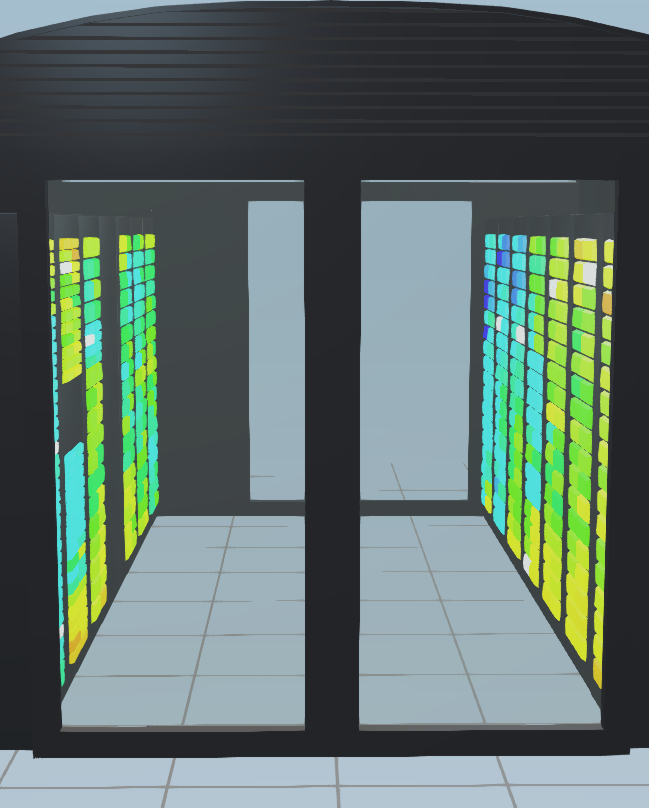
\includegraphics[width=\linewidth]{3d-model}
  %\includegraphicsvg[width=\linewidth]{sohpc-logo}
  \thispagestyle{empty}
\end{minipage}
\vskip 30pt
\frenchspacing
\begin{multicols}{3}

\lettrine[lines=4,nindent=0em]{\highlight{T}}{}he current monitoring system\cite{current} consists of several layers which allow to aggregate in a single point heterogeneous data sources which consist of computing elements, node, job scheduler and facility telemetry of the Galileo supercomputer located at CINECA, Bologna, Italy.

The system was named \textit{ExaMon}\footnote{Shorthand for Exascale Monitoring} and is built on top of MQTT protocol\cite{mqtt} which allows measured metrics to be send to a central broker where received data are processed and stored in KairosDB\cite{kairos} database utilizing Cassandra cluster.

\begin{figure}[H]
%\color{yellow}\rule{\linewidth}{3cm}\color{black}
    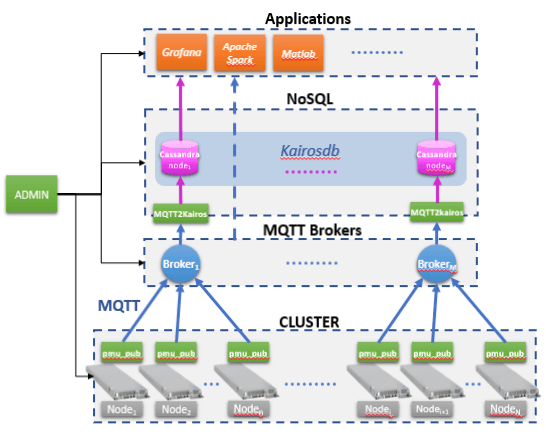
\includegraphics[width=0.9\linewidth]{examon-architecture}
    \caption{Examon Architecture}
    \label{arch}
\end{figure}

This enables us to post-process data in time-oriented fashion in order to visualise them on a time-line and as a single number as well.

Current implementation uses Grafana framework to visualise data stored in KairosDB. Grafana will be replaced by the project's result of creating a dedicated web application for defined use-cases with 3D model of a cluster room showing various metrics of the whole HPC system with focus on energy consumption and efficiency.

\section*{Methods}
The whole project can be separated into three phases. First phase is data anylysis where the whole dataset of available metrics was presented, how they are distributed and eventually processed on the back-end.

Datasets can be divided into multiple levels of aggregation:
\begin{itemize}
    \item{Per-core level -- the most low-level data can be found in core's registers such as IPS, Lx-cache misses and more. It also provides info about its load and temperature.}
    \item{Per-CPU level -- each node consists of two CPUs and each of them can provide data about its C-states, energy counters and its frequency.}
    \item{Per-node level -- most of the information available on node-level basis are coming from IPMI\cite{ipmi}. Via this interface we can access info about node's utilization, multiple temperature sensors and average power consumption.}
    \item{Per-cluster level -- the Galileo's cluster room was equipped with several environmental sensors. This dataset is not currently available due to technical problems.}
    \item{Per-job level -- data gathered using the PBS scheduler's hooks. This dataset is aside from previous ones since it points to allocated and used resources of the job submitted to the queue. This data are stored directly to Cassandra cluster ommitting KairosDB.}
\end{itemize}

With each level we can aggregate the lower levels (except job-level data). This is especially useful for core-level data which are mostly too dense for any comprehensible visualisation.

Second phase was to visualize data stored in KairosDB in simple yet insightful way in a lightweight web application. The application, called ExaMon Web, uses Angular framework as its base on top of which several other libraries were used. Worth mentioning are Dygraphs and Bootstrap. The former library produces powerful time-oriented charts utilizing the canvas element in web browser. The latter is a CSS framework to produce uniform user interface across the whole application.

Compared to Grafana, the created web application feels more lightweight, fast and easier to use because of the prepared datasets which are being used. The balance between configurability and the ease of use must have been found. We concluded the best way to achieve this was to enable time selection on given datasets but restrict configurability of the charts themselves. This way user is not bogged down with configuration and only focuses on prepared data. If there is such desire to see other metrics the Grafana framework is still available right next to the ExaMon Web. As an additional feature, compared to Grafana, we can perform more advanced queries using the KairosDB REST API.

The last phase was to utilize the live stream of MQTT messages right in the ExaMon Web. Two use-cases were defined for the MQTT messages depending on their origin.

Several job info MQTT messages are send during the job's lifecycle inside the PBS and every job is assigned a unique job ID. Using the ID user can subscribe to given messages and view various information on the ExaMon Web job dashboard. The dashboard also uses Cassandra cluster in case the job is already finished and stored in the cluster. This way user can see additional data about their job.

Using the job data user can view detailed info about allocated resources of the given job such as CPU load, system utilization and more as seen in \ref{pic:job-perf}.

Second use-case is


\section{Results}
\section{Discussion \& Conclusion}

You can use your blog posts as a basis for this report.

Graphics should be your own. Short title should be just few words. Highlight word or two to give some separation within the short title. Long name preceding short title is not necessarily the title of your project as facts about the projects, mentors and the author(s) are given at the end. Usually in magazines no two articles are the same in terms of formatting. You are free to do figure positioning and column spans. Bear in mind that with multiple columns spanning in \LaTeX is non-trivial.

Example nearby shows how wrapfig can be used for spanning into two columns. Don't be afraid of large screenshots. To get an idea on the style take a look into PRACE digest, newsletter and other popular scientific texts available on Internet. Google for \highlight{writing popular scientific}. For example: \url{http://awelu.srv.lu.se/genres-and-text-types/writing-in-academic-genres/popular-science-writing/}

\section*{Paper format}
We use A4 paper size with 10pt Charter or Georgia font. Text at the end and captions should be 9pt. Short title Helvetica (Arial) medium or light 45pt with 50pt spacing. Long title and Abstract 12pt. Margins should be 12mm everywhere except ob the bottom where 0.75 inch is reserved for page number. Other important dimensions: 
\begin{description}
  \item[column separation]  \the\columnsep
  \item[column width] \the\columnwidth
  \item[textwidth] \the\textwidth
\end{description}
For compiling \LaTeX it is recommended (if having troubles) to use latest \TeX live distribution. Use pdf\LaTeX instead of classical \LaTeX as it outputs PDF directly, wraps URLs correctly and can include PNG files directly. Do not use JPEG for screenshots! JPEG is for photos only. For sketching use \href{http://www.inkscape.org}{Inkscape}. 

\section*{General guidelines}
\newcommand{\itempar}[1]{\noindent\highlight{\textsf #1}\par\noindent}
\begin{itemize}
  \setlength{\itemsep}{0pt plus 3pt}\setlength{\topsep}{0pt plus 4pt}
  \setlength{\partopsep}{0pt}\setlength{\parsep}{0pt}\setlength{\parskip}{0pt}
\item All articles should be in English.
\item Articles should be a maximum of 3 pages.
\item All articles should contain at least 2 images.
\end{itemize}

\itempar{Who Am I writing for?}This article should be in the style of a popular science article. This means that is should be relatively simple to understand and entertaining. 


\noindent The audience are not specialists in the field in questions, but rather interested laypeople. Adapt your content to the level of general knowledge of an educated adult who is not a computer scientist or scientist in your field Let your enthusiasm for your project show! Explain terms well. 

\noindent Use vivid language. Use illustrations, graphics and examples.

\itempar{Formatting}%
Final formatting will consist of a three column article 2-3 pages long. Please follow the formatting in the templates. Please provide links to hi-res version of any images submitted.

\itempar{Title}%
This should succinctly describe the content of the article. Be descriptive!
%

The title should be at the top of your first page and centred.
Do not use a title page.
%Headings with an asterisk(*) must be included

\itempar{Content}%
The following is the suggested content of the article. You do not have to include section heading to match, but should match the general flow and content.

\itempar{Author}
Author's names and institutional affiliation at the end.

\itempar{Abstract -- What did I do - in brief}  An abstract is a one-paragraph summary of the entire article. It should describe the question/problem or research topic addressed in the project and the methods used to answer or explore this area. It should highlight the important parts of the article. This is easiest to write once you have completed the rest of the article. Include a sentence summarising the introduction, methods, results and discussion section. The abstract should not contain citations. Equations should be avoided if possible. And not numbered if not referenced in text. 

\itempar{Introduction -- What is the project?}%
The introduction should describe the question/problem/research area addressed by the project and set the context for your work. It should explain why your project is interesting or important. It should introduce the techniques and approach you used to complete the project.

\itempar{Methods -- How did I complete the project?}%
Briefly describe what was actually done. This should include more detail on techniques and approaches, with enough detail that an interested person could attempt to reproduce your work (You do not have to include every detail, but use citations to give the required background). 

\itempar{Results -- What did I find out?}%
Focus on what worked! Outline the outcomes and results of your project

\itempar{Discussion \& Conclusion}
(What does that mean?) Explain your conclusions and your interpretation of your results. How did it compare to what was to be expected or previous work? What implications does this have for other work?

\itempar{References} (what work did I reference?)

\itempar{Acknowledgements} (who helped me?) PRACE acknowledgement will be given together at the colophon. Site acknowledgement if required. Other acknowledgement if requested.
%\multicolinterrupt{\textcolor{prace-darkblue}{\lipsum[16]}}

\subsection*{Tables and Figures}
%Strange why the following macro needs to be repeated due to multicolinterrupt
%\newcommand{\itempar}[1]{\noindent\highlight{\textsf #1}\par\noindent}

Week 3 plans are given separately and contain the following items:

\itempar{Workplan} Please append and up-to-date workplan (Week 3 reports) outlining what you did week by week. Introduction can be used for final report too.

\itempar{Appendices} (Extra information)
Optional --- anything else you want to include, but not publish

\noindent\begin{minipage}[H]{2\columnwidth+\columnsep}
 %\vspace{-15pt}
  \begin{figure}[H]
  \centering
  \color{yellow}\rule{\linewidth}{3.8cm}\color{black}
  %\includegraphics{}
  \caption{Captions for figures should be used only if necessary and referenced in text.}
\label{fig:my_label}
\end{figure}
\end{minipage}

\itempar{Appendices} (Compulsory)

\itempar{Award statement}%
Please amend a section to ``Week 3 plans'' at end of the programme stating why you think you should win
\begin{enumerate}
  \item The HPC Ambassador Award.
  \item The Best Visualisation Award.
\end{enumerate}
Information given as an update will be used to aid reviewers in evaluation of the projects and will not be publicly available.



\subsection*{Tables and Figures}

All tables and figures should be captioned. All tables and figures should be put into context in the text. Give your main figure instead of SoHPC logo figure nearby the title. Tables and figures should sequentially numbered. Make sure that there isn't a page break in the middle. Sometimes it is easier to add more text to get good balancing between columns.



\itempar{Acronyms, technical terms}%
Symbols, abbreviations and acronyms should be defined the first time they are used and then used consistently from there on. Note that too technical slang is not desired here.


\begin{table}[H]
 \caption{Random table}
 \centering
 \begin{tabular}{llr}
 \toprule
 \multicolumn{2}{c}{Name} \\
 \cmidrule(r){1-2}
 First name & Last Name & Grade \\
 \midrule
 John & Doe & $7.5$ \\
 Richard & Miles & $2$ \\
 \bottomrule
 \end{tabular}
\end{table}

%\vspace*{5cm}

\begin{figure*}[t]
  \color{yellow}\rule{2\columnwidth+\columnsep}{10cm}%
  %\includegraphics[width=2\columnwidth+\columnsep]{fig4}
  \hspace{\columnsep}
  \begin{minipage}[b]{1.0\columnwidth}
    \color{yellow}\rule{\linewidth}{4.6cm}\\[\columnsep]
    \color{prace-lightblue}\rule{\linewidth}{5cm}
    % \includegraphics[width=\linewidth]{fig5}
    % \includegraphics[width=\linewidth]{fig6}
  \end{minipage}
  \color{black}
  \vspace{-3ex}
  \caption*{Large figures should be placed at top and can be combination of
    several sub-figures. With or without caption. Do not number figures if
    they are not referenced in text. Several sentences can be used to
    describe the figures.}
  \label{fig:large}
\end{figure*}
%\noindent Answers to the questions of general interest will be published at the page \url{http://trac.lecad.fs.uni-lj.si/sohpc/wiki/template} where also all template files are available for download.

\section*{Videos and final presentations}
We recommend that videos are prepared in \href{https://support.google.com/youtube/answer/1722171}{720p HD resolution} (19:6). Screen casts can be recorded by \href{http://atomisystems.com/activepresenter/free-edition/}{Active Presenter --  free edition}.

It is advisable that you prepare a text that you will be recording along with the presentation.\vspace{50mm} For quick check of how recording goes try the following:
\begin{enumerate}
 \setlength{\itemsep}{0pt}\setlength{\parskip}{0pt}
 \item Enter Full Motion Recording (FMR).
 \item Select Custom resolution (1280x720) and portion of screen you will be capturing.
\item Disable Floating Toolbar (bottom left).
\item Unmute microphone on the desktop.
\end{enumerate}
Once a capture has finished, one can:
\begin{itemize}
  \item Edit the capture (Cut, delete, copy, part of the captured video)
  \item Insert text, shapes, spotlights, higlight boxes, images
  \item Other elements possible.
  \item Each added feature appears in the timeline and you can edit for how long it will appear, where it will appear and how it will appear/disappear through transitions
  \item Position of these can also be altered to give a sense of ``animation''.
  \item Export it into MP4 or AVI format.
\end{itemize}
There are many other ways to record a screen and edit such as \href{http://geekthis.net/blog/98/virtualbox-video-capture}{VirtualBox screen recording} and \href{https://youtu.be/WDh1CrL2344}{Windows Movie Maker}. For video encoding one can use \href{http://www.erightsoft.com/SUPER.html}{Super~\copyright} or similar software. Please visit examples of \href{https://www.youtube.com/playlist?list=PLhpKvYInDmFWy66381nifGkCJBLb6iwGf}{SoHPC 2016 videos} on Youtube.


\section*{Section 1}
Section names should not be too technical. No numbering should be used. Sections can be even questions for the text that follows. Section names can state the fact explained in continuation.

\begin{figure}[H]
  \color{yellow}\rule{\linewidth}{3cm}\color{black}
  % \includegraphics[width=\linewidth]{vortex}
  \caption{Quickly explain the content of the figure if you reference it in
    the text.}
  \label{fig:vortex}
\end{figure}


%\subsection*{Subsection 1}
\begin{align}
 A = 
 \begin{bmatrix}
 A_{11} & A_{21} \\
 A_{21} & A_{22}
 \end{bmatrix}
 \end{align}
Please balance the size of figures and text in such way that you will have the complete page filled. It should not be half way ended. Use citations as superscript\cite{Figueredo:2009dg} if absolutely necessary.
\newcommand{\sohpcinfo}[1]{\par\vspace{1ex}\footnotesize
  \textcolor{prace-lightblue}{PRACE SoHPC}%
  \textcolor{prace-darkblue}{#1}\\[0.5ex]\scriptsize
}

\renewcommand\refname{\usefont{OT1}{phv}{m}{n}\selectfont\small{References}}
\begin{thebibliography}{9}
\vspace*{-1ex}  % adjust this
\scriptsize
\bibitem[1]{current}
Beneventi, Francesco, et al. "Continuous learning of HPC infrastructure models using big data analytics and in-memory processing tools." 2017 Design, Automation \& Test in Europe Conference \& Exhibition (DATE). IEEE, 2017.

\bibitem[2]{mqtt}
Locke, Dave. "Mq telemetry transport (mqtt) v3.1 protocol specification." IBM developerWorks Technical Library (2010).

\bibitem[3]{kairos}
Goldschmidt, Thomas, et al. "Scalability and robustness of time-series databases for cloud-native monitoring of industrial processes." Cloud Computing (CLOUD), 2014 IEEE 7th International Conference on. IEEE, 2014.

\bibitem[4]{ipmi}
Kaufman, Gerald J. "System and method for application programming interface for extended intelligent platform management." U.S. Patent No. 7,966,389. 21 Jun. 2011.
APA
\end{thebibliography}

\vfill
\noindent\begin{minipage}[b]{0.7\linewidth}
\begin{flushleft}
  \usefont{OT1}{phv}{m}{n}\selectfont
  \sohpcinfo{Project Title}
  \href{https://summerofhpc.prace-ri.eu/web-visualization-of-energy-load-of-an-hpc-system/}{Web visualization of Energy load of an HPC system}
  
  \sohpcinfo{Site}
  CINECA, Italy
  
  \sohpcinfo{Authors}
  \href{mailto:xstehl14@stud.fit.vutbr.cz}{\theauthor},
  BUT, Czech Republic
  
  \sohpcinfo{Mentor}
  \href{mailto:a.bartolini@unibo.it}{Dr. Andrea Bartolini}, UNIBO, Italy
\end{flushleft}
\end{minipage}\hfill%
\begin{minipage}[b]{0.3\linewidth}
  \color{prace-darkblue}\rule{\linewidth}{2.5cm}\par
  \tiny\theauthor
\end{minipage}%
\vspace{-1.5ex}% any of information below is optional
\begin{flushleft}
  \sohpcinfo{ More Information}
  \href{http://www.virtouso.org}{www.virtouso.org}
  \sohpcinfo{ Acknowledgement}
  Write any requested acknowledgements or thanks here. Mentors should be
  asked for them too.

    \sohpcinfo{ Project ID} 1705
\end{flushleft}
\end{multicols}
\end{document} 

%%Local Variables:
%%% mode: latex
%%% TeX-parse-self: t
%%% TeX-auto-save: t
%%% TeX-source-specials-mode: t
%%% TeX-PDF-mode: t
%%% LaTeX-command: "pdflatex -synctex=1  --enable-write1"
%%% TeX-master: t
%%% ispell-local-dictionary: "british"
%%% End:

